\graphicspath{{img/appendix}{img/impl}}

\newcommand\invisiblesection[1]{%
  \refstepcounter{chapter}%
  \addcontentsline{toc}{chapter}{\protect\numberline{\thechapter}#1}%
  \sectionmark{#1}}

\invisiblesection{Hyperparameter Optimization}
\subsubsection{Hyperparameter Optimization Plots (moving avg. of 8)}
\label{app:hyperparam_optim}
\begin{figure}[H]
    \advance\leftskip-2.3cm
    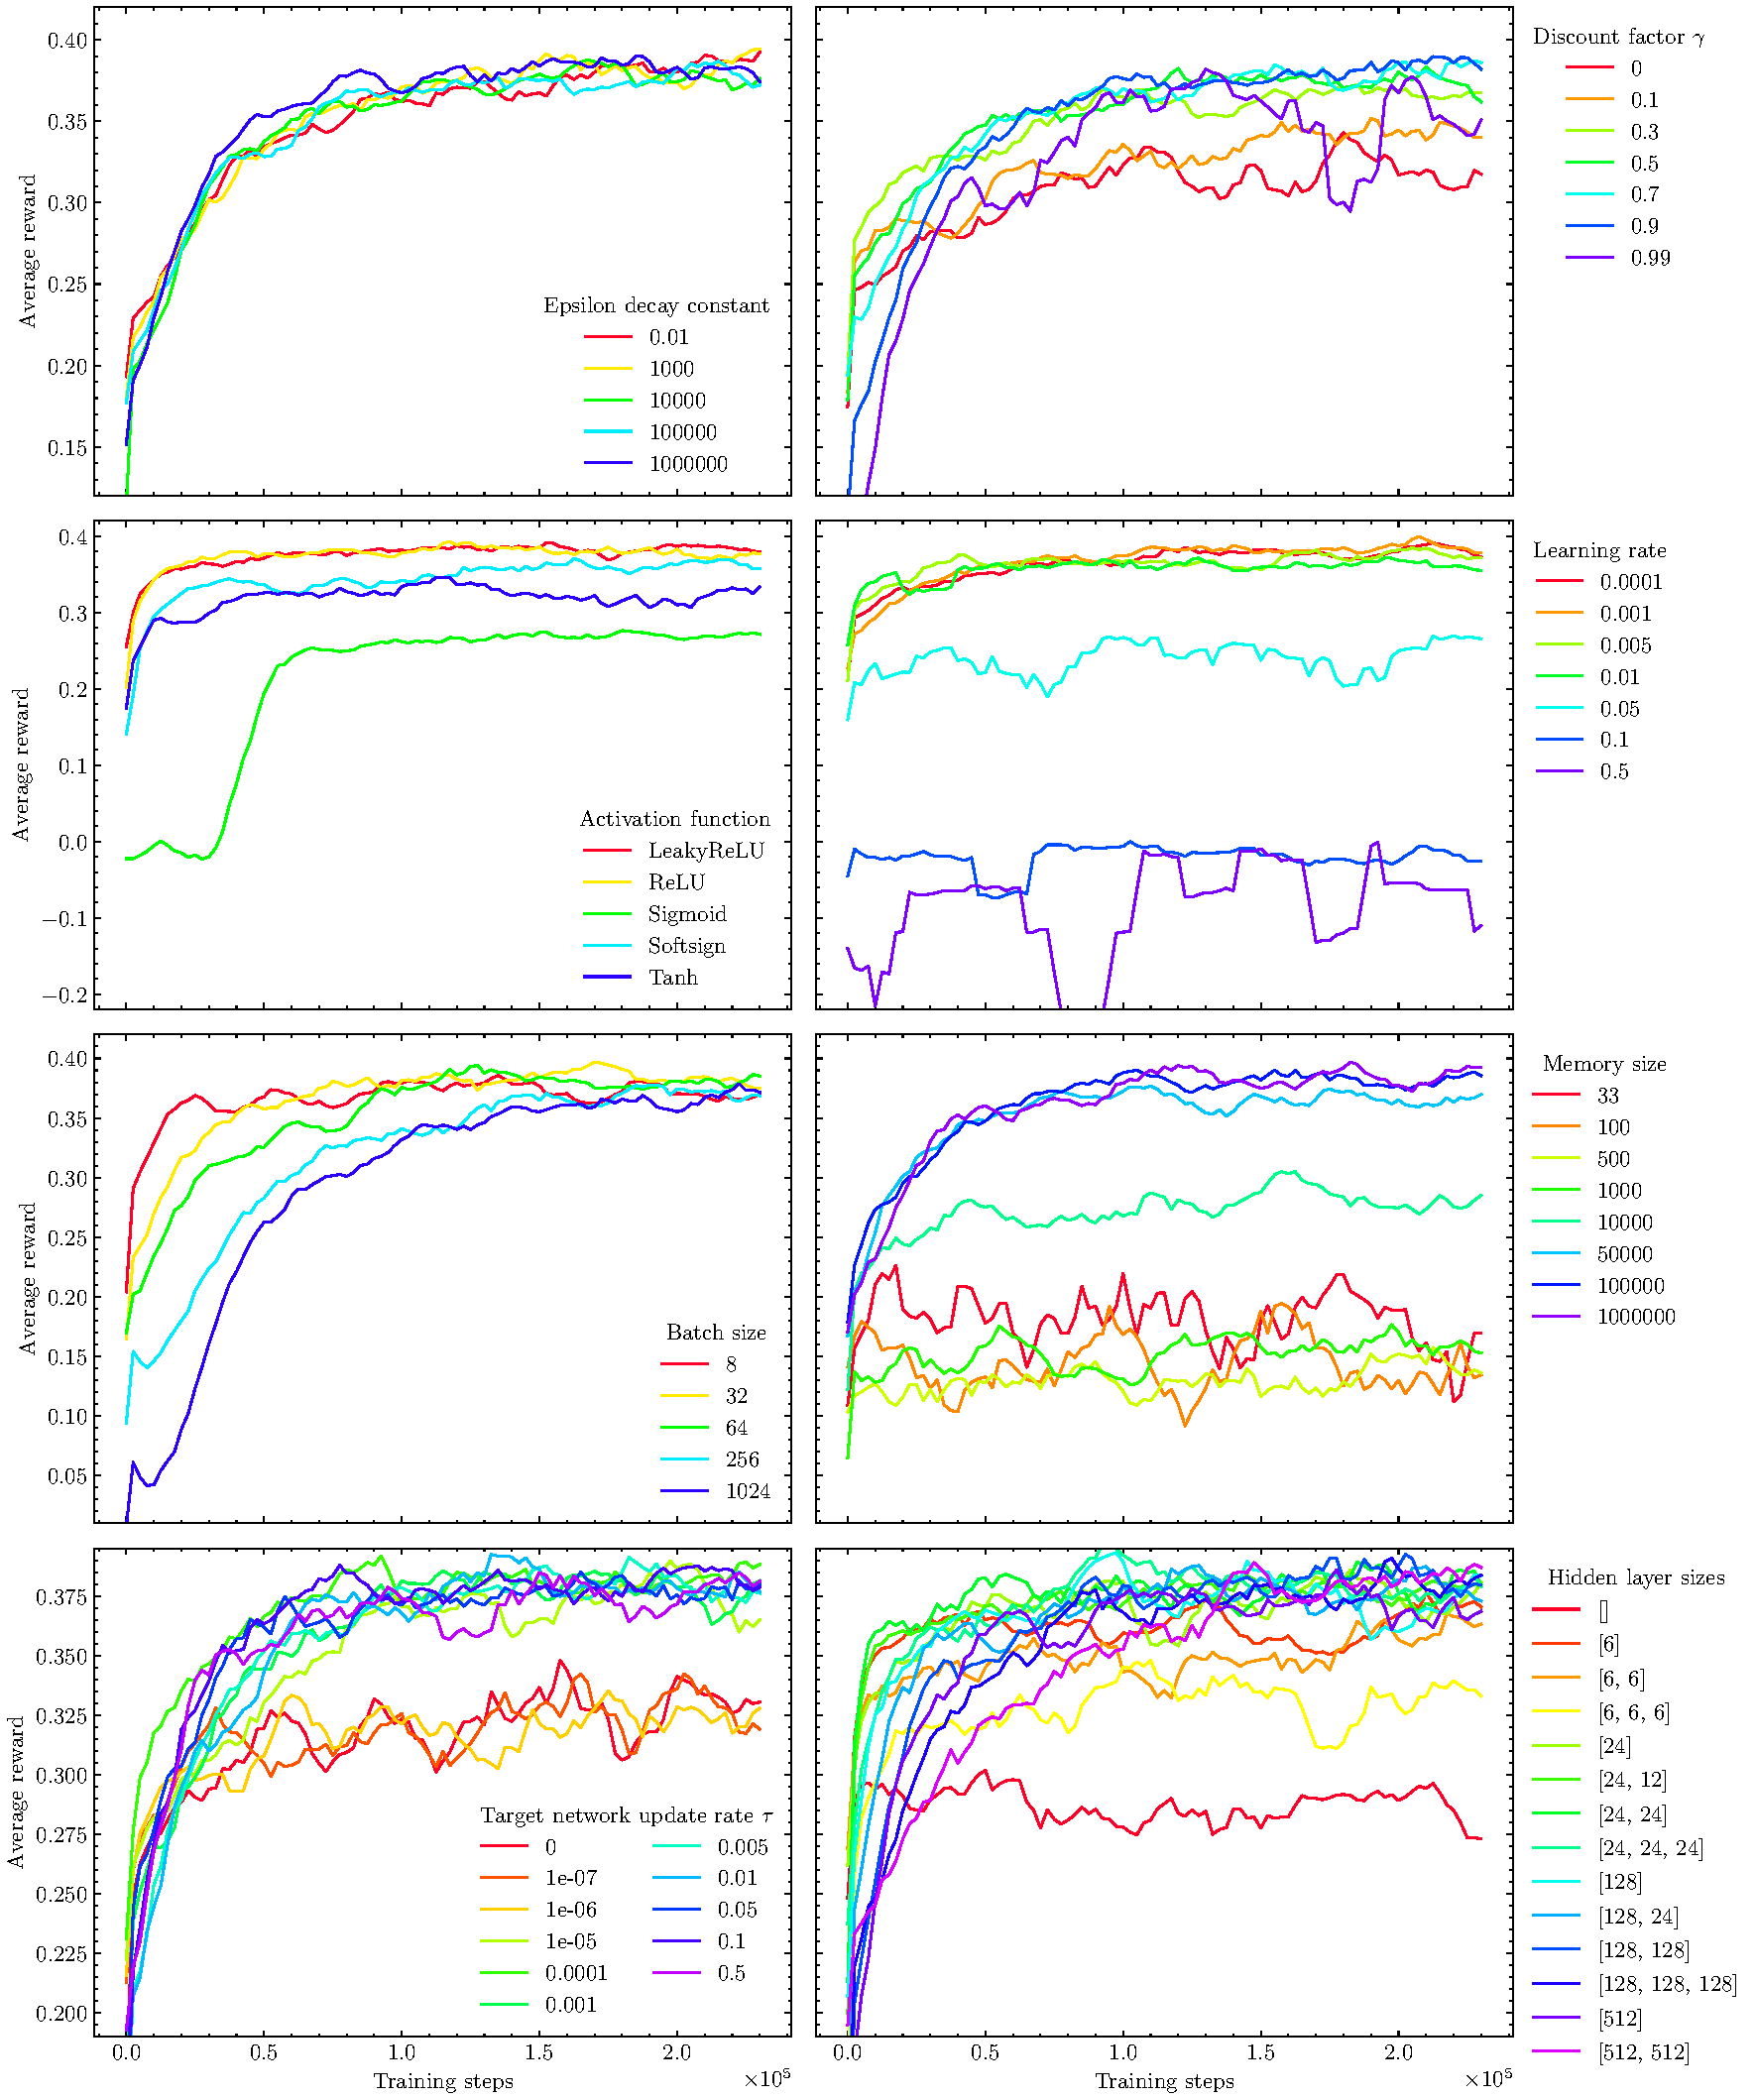
\includegraphics[width=1.28\textwidth]{hyperparam_optim_8_sci.pdf}
    \caption{Hyperparameter optimization plots analyzed in section \ref{sec:hyperparam_optim}.}
    \label{fig:hyperparam_optim_8}
\end{figure}

\subsubsection{Hyperparameter Optimization Plots (moving avg. of 30)}
\label{app:hyperparam_optim_30}
\begin{figure}[H]
    \advance\leftskip-2.3cm
    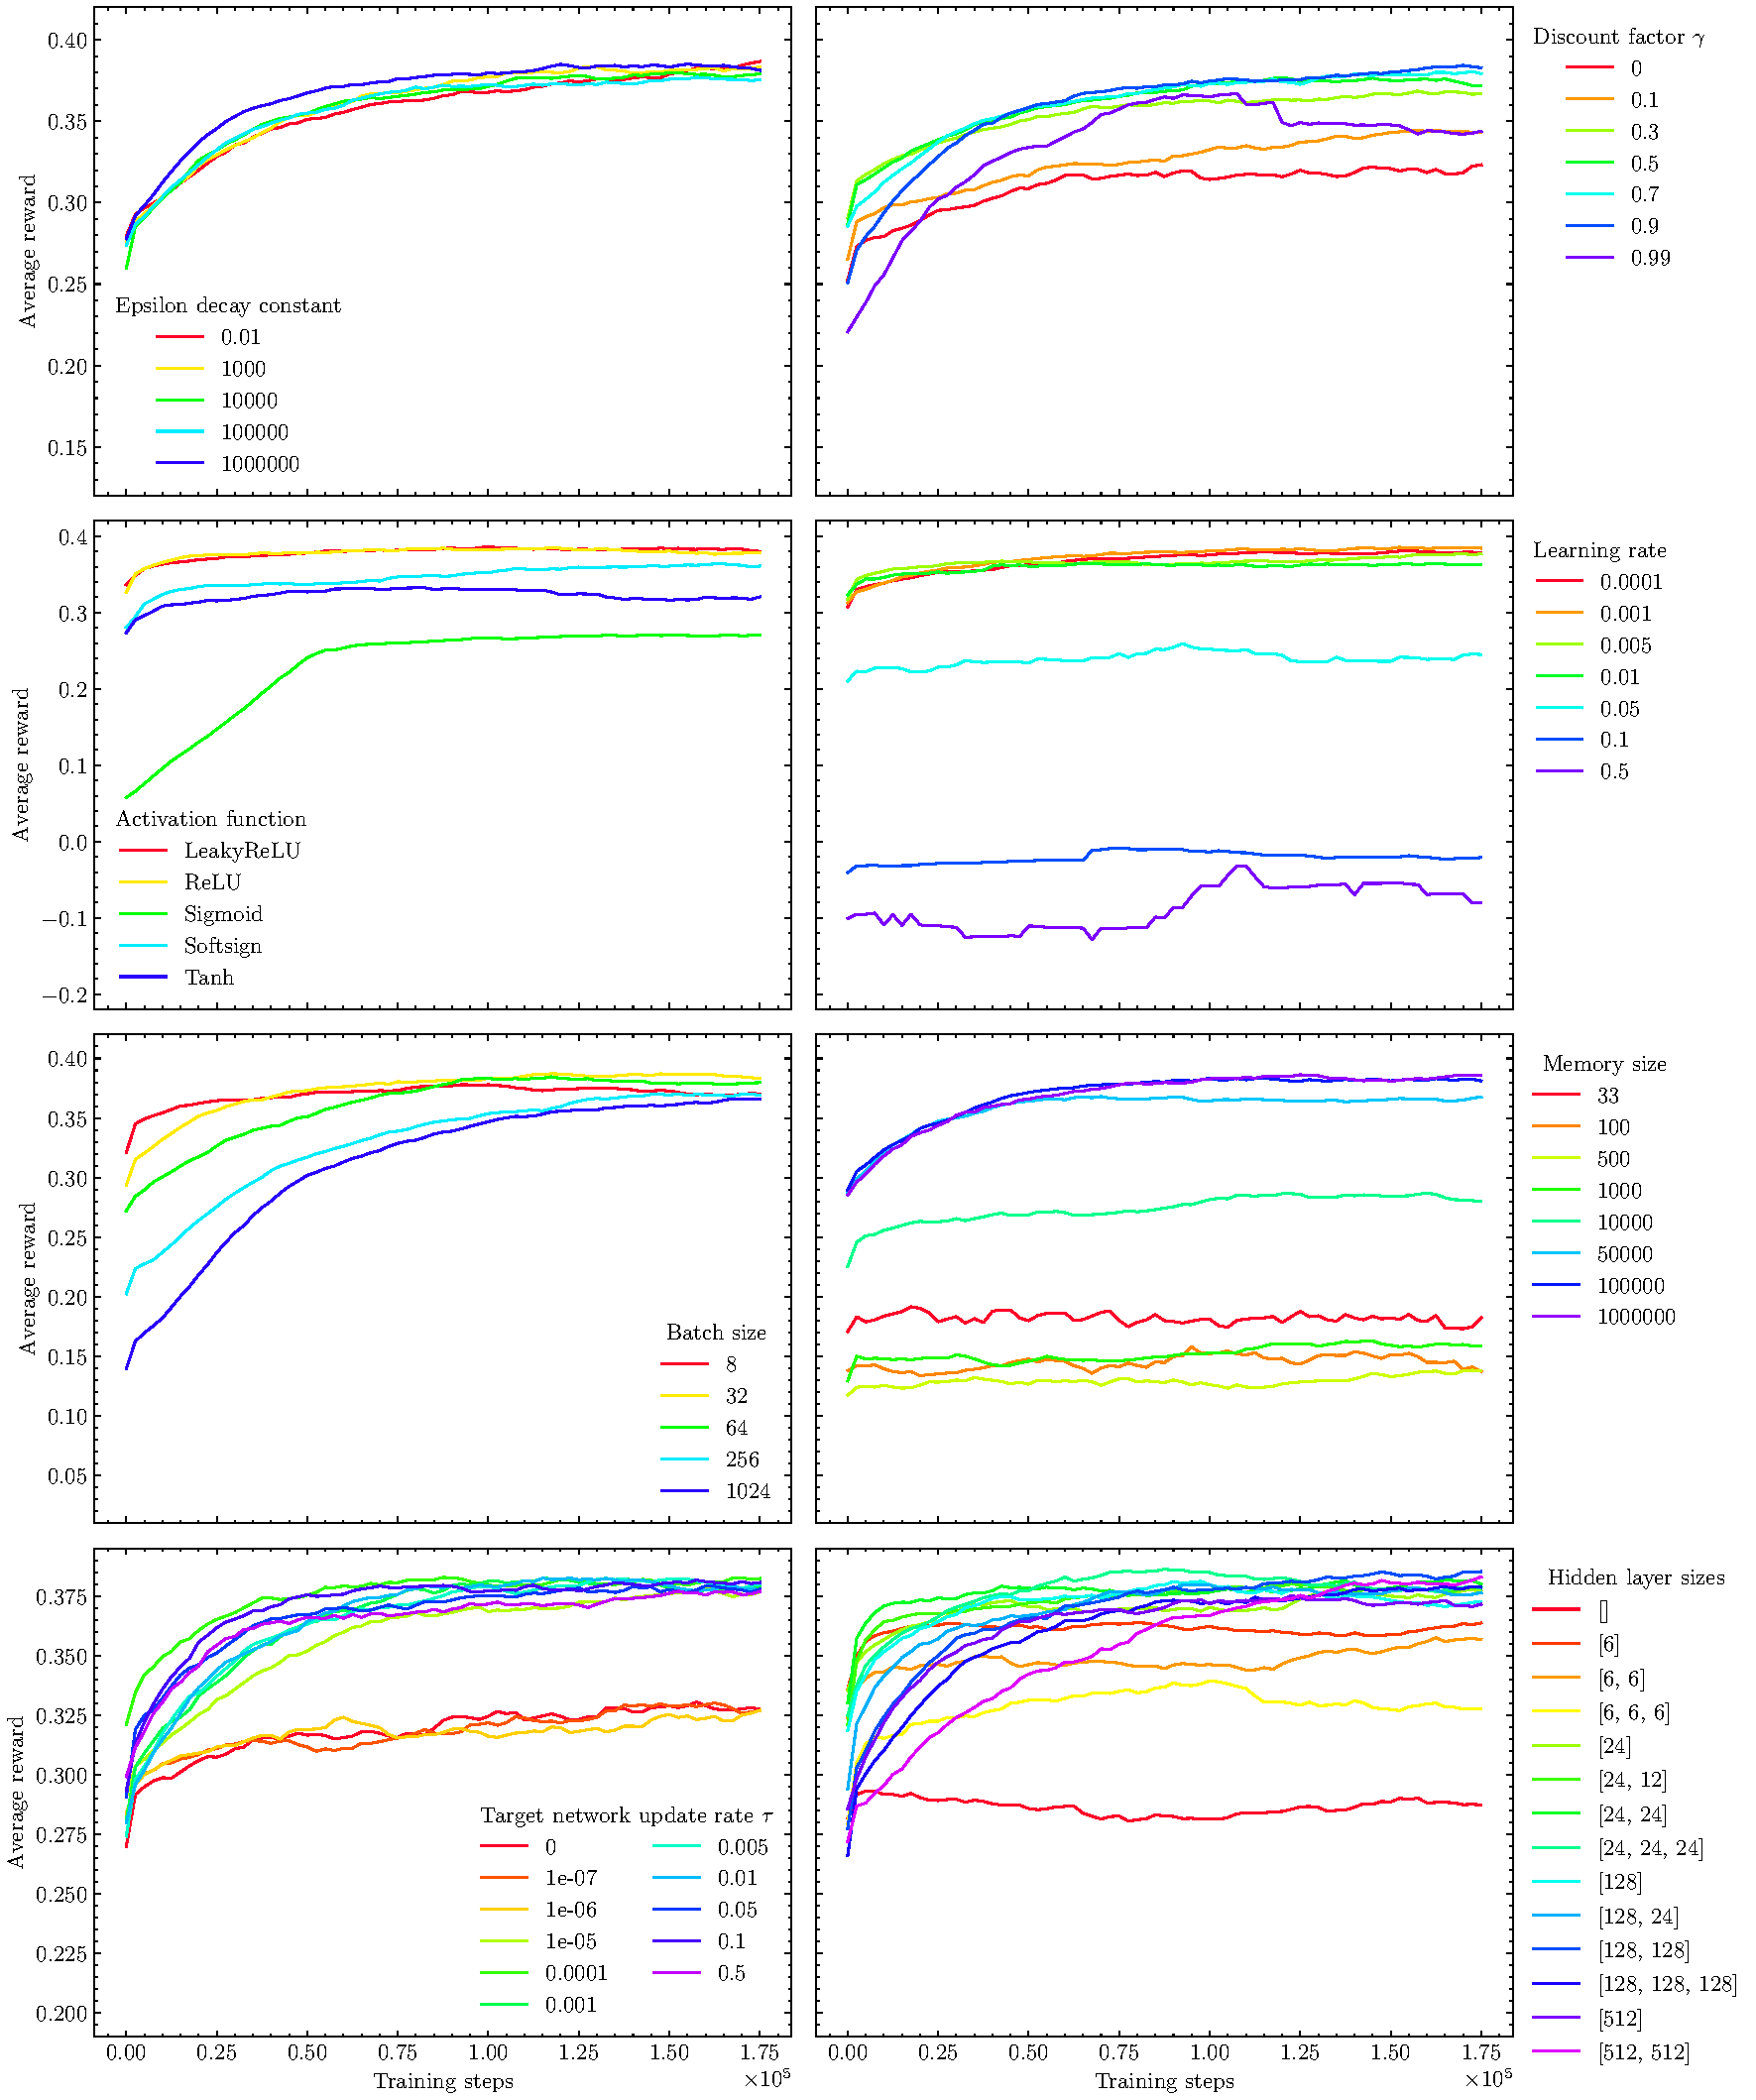
\includegraphics[width=1.28\textwidth]{hyperparam_optim_30_sci.pdf}
    \caption{Hyperparameter optimization plots analyzed in section \ref{sec:hyperparam_optim}.}
    \label{fig:hyperparam_optim_30}
\end{figure}


\chapter{Code}
\label{app:code}

This appendix contains the code that is needed to reproduce the results presented in this thesis. The code depends on the \texttt{smarttasep} package, which can be installed on your system (or in a virtual environment) after setting up the python interpreter by running 
\begin{minted}
    [bgcolor=LightGray, fontsize=\footnotesize]
    {bash}
  python -m pip install smarttasep
\end{minted}
On some systems, the \texttt{python} command might be replaced by \texttt{python3} or \texttt{py}. The library's source code can be found at \cite{maertens_smarttasep_github_2023}.
\\
\\
Only the code for running the training is shown here. After training, the model is automatically saved and the unique model ID is printed to the console. Models can be evaluated by running the simulation:
\begin{minted}
    [bgcolor=LightGray, fontsize=\footnotesize]
    {python}
from smarttasep import Trainer

trainer = Trainer.load(model_id=1, total_steps=1_500_000)

trainer.run(reset_stats=True)
\end{minted}
or by launching the \texttt{Playground}:
\begin{minted}
    [bgcolor=LightGray, fontsize=\footnotesize]
    {python}
from smarttasep import Playground

Playground(model_id=1)

\end{minted}


\section{First training: Equal Speeds}
\label{app:first_training}
\begin{minted}
    [bgcolor=LightGray, fontsize=\footnotesize, linenos, breaklines]
    {python}
  from smarttasep import Trainer, Hyperparams, EnvParams

  if __name__ == '__main__':
      envParams = EnvParams(render_mode="human",
                            length=128,
                            width=24,
                            moves_per_timestep=200,
                            window_height=200,
                            observation_distance=3,
                            distinguishable_particles=True,
                            initial_state_template="checkerboard",
                            social_reward=True,
                            use_speeds=True,
                            sigma=0.0001,
                            allow_wait=True,
                            invert_speed_observation=True,
                            speed_observation_threshold=0.35)

      hyperparams = Hyperparams(BATCH_SIZE=32,
                                GAMMA=0.85,
                                EPS_START=0.9,
                                EPS_END=0.05,
                                EPS_DECAY=100_000,
                                TAU=0.005,
                                LR=0.001,
                                MEMORY_SIZE=500_000)
  
      trainer = Trainer(envParams, hyperparams, reset_interval=100_000,
                        total_steps=500_000, do_plot=True, plot_interval=4000, new_model=True)
  
      trainer.train_and_save()
\end{minted}

\section{Second training: Uniformly Distributed Speeds, Simple Reward}
\label{app:second_training}
\begin{minted}
    [bgcolor=LightGray, fontsize=\footnotesize, linenos, breaklines]
    {python}
from smarttasep import Trainer, Hyperparams, EnvParams

if __name__ == '__main__':
    envParams = EnvParams(render_mode="human",
                          length=128,
                          width=24,
                          moves_per_timestep=200,
                          window_height=200,
                          observation_distance=3,
                          distinguishable_particles=True,
                          initial_state_template="checkerboard",
                          social_reward=True,
                          use_speeds=True,
                          sigma=10,
                          allow_wait=True,
                          invert_speed_observation=True,
                          speed_observation_threshold=0.35)

    hyperparams = Hyperparams(BATCH_SIZE=32,
                              GAMMA=0.85,
                              EPS_START=0.9,
                              EPS_END=0.05,
                              EPS_DECAY=100_000,
                              TAU=0.005,
                              LR=0.001,
                              MEMORY_SIZE=500_000)

    trainer = Trainer(envParams, hyperparams, reset_interval=100_000,
                      total_steps=500_000, do_plot=True, plot_interval=4000, new_model=True)

    trainer.train_and_save()
\end{minted}


\section{Global Structures - The Easy Way}
Edit the \texttt{speed\_gradient\_linearity} parameter as needed.
\begin{minted}
    [bgcolor=LightGray, fontsize=\footnotesize, linenos, breaklines]
    {python}
from smarttasep import Trainer, Hyperparams, EnvParams

if __name__ == '__main__':
    envParams = EnvParams(render_mode="human",
                          length=128,
                          width=32,
                          moves_per_timestep=80,
                          window_height=300,
                          observation_distance=3,
                          distinguishable_particles=True,
                          initial_state_template="checkerboard",
                          social_reward=False,
                          use_speeds=True,
                          sigma=5,
                          allow_wait=True,
                          invert_speed_observation=True,
                          speed_observation_threshold=0.35,
                          punish_inhomogeneities=False,
                          speed_gradient_reward=True,
                          average_window=2000,
                          speed_gradient_linearity=100)

    hyperparams = Hyperparams(BATCH_SIZE=128,
                              GAMMA=0.99,
                              EPS_START=0.9,
                              EPS_END=0.05,
                              EPS_DECAY=50_000,
                              TAU=0.005,
                              LR=0.005,
                              MEMORY_SIZE=900_000)

    trainer = Trainer(envParams, hyperparams, total_steps=900_000, new_model=false)

    trainer.train_and_save()
\end{minted}

\section{Global Structures - The Nice Way}
\begin{minted}
    [bgcolor=LightGray, fontsize=\footnotesize, linenos, breaklines]
    {python}
from smarttasep import Trainer, Hyperparams, EnvParams

if __name__ == '__main__':
    envParams = EnvParams(render_mode="human",
                          length=100,
                          width=10,
                          moves_per_timestep=200,
                          window_height=100,
                          observation_distance=4,
                          distinguishable_particles=True,
                          density=0.4,
                          use_speeds=True,
                          sigma=5,
                          allow_wait=false,
                          invert_speed_observation=True,
                          speed_observation_threshold=0.35,
                          punish_inhomogeneities=True,
                          inh_rew_idx=0,
                          speed_gradient_reward=False,
                          average_window=4000,
                          binary_speed=True)

    hyperparams = Hyperparams(BATCH_SIZE=64,
                              GAMMA=0.8,
                              EPS_START=0.9,
                              EPS_END=0.05,
                              EPS_DECAY=150_000,
                              TAU=0.005,
                              LR=0.005,
                              MEMORY_SIZE=500_000)

    trainer = Trainer(envParams, hyperparams, total_steps=1_500_000, new_model=True, random_density=False, diff_models=True, num_models=2)

    trainer.train_and_save()
\end{minted}